\documentclass[11pt,a4paper,oneside]{article}

% use % use % use \input{template} to include in your document

\usepackage[utf8]{inputenc}
\usepackage[english]{babel}
\usepackage[nottoc]{tocbibind}
\usepackage[cm]{fullpage}
\usepackage[table,xcdraw]{xcolor}
\usepackage{graphicx}
\usepackage{fancyhdr}
\usepackage{helvet}
\usepackage{tabularx}
\usepackage{listings}
\usepackage{xcolor,mdframed}
\usepackage{hyperref}
\usepackage{float}
\usepackage{multirow}
\usepackage[nonumberlist,acronym,toc]{glossaries}
\usepackage{lscape}
\usepackage{indentfirst}
\usepackage{caption}
\usepackage{charter}
\usepackage[T1]{fontenc}
\usepackage{wasysym}
\usepackage{ifthen}
\usepackage{lastpage}
\usepackage{subfig}

\makeatletter

\pagestyle{fancy}

% tables
\def\arraystretch{1.5}
\restylefloat{table}
\newcolumntype{L}{>{\raggedright\arraybackslash}p}
\newcolumntype{R}{>{\raggedleft\arraybackslash}p}

% colors
\definecolor{dkgreen}{rgb}{0,0.6,0}
\definecolor{gray}{rgb}{0.5,0.5,0.5}
\definecolor{mauve}{rgb}{0.58,0,0.82}

% link
\hypersetup{%
	colorlinks=true,
	linkcolor=black,
	filecolor=gray,
	urlcolor=gray,
	breaklinks=true
}
\urlstyle{same}

% code
\lstset{%
	frame=single,
	language=bash,
	aboveskip=3mm,
	belowskip=3mm,
	numbers=none,
	showstringspaces=false,
	columns=flexible,
	basicstyle={\small\ttfamily},
	keywordstyle=\color{blue},
	commentstyle=\color{dkgreen},
	stringstyle=\color{mauve},
	breaklines=true,
	breakatwhitespace=false
	tabsize=2
}

% add parameters for Nginx configuration
\lstdefinelanguage{Nginx}{
	morekeywords={
		server,server_name,listen,rewrite,location,
		ssl,ssl_session_cache,ssl_session_timeout,ssl_certificate,ssl_certificate_key,ssl_protocols,ssl_ciphers,ssl_verify_depth,
		access_log,error_log,error_page
	}
}

% add parameters for Ini files
\lstdefinelanguage{Ini}{
	tag=[s]{[]},
	tagstyle=\color{mauve},
	usekeywordsintag=true
}[html]

% add parameters for JSON files
% \lstdefinelanguage{JSON}{
	% tag=[s]{[]},
	% usekeywordsintag=true
% }[html]

% add some keywords to bash language
\lstset{language=bash}
\lstset{
	morekeywords={
		cp,mkdir,rm,ln,unlink,chown,chmod,sudo,
		usermod,useradd,userdel,passwd,
		hostname,tar,gzip,crontab,wget,nginx,mysql
	}
}

% nice boxes
\newenvironment{important}[1][]{%
	\begin{mdframed}[%
	backgroundcolor={red!15}, hidealllines=true,
	skipabove=0.7\baselineskip, skipbelow=0.7\baselineskip,
	splitbottomskip=2pt, splittopskip=4pt, #1]%
	\makebox[0pt]{% ignore the withd of !
		\smash{% ignore the height of !
			\fontsize{32pt}{32pt}\selectfont% make the ! bigger
			\hspace*{-19pt}% move ! to the left
			\raisebox{-2pt}{% move ! up a little
				{\color{red!70!black}\sffamily\bfseries !}% type the bold red !
			}%
		}%
	}%
}{\end{mdframed}}

\newenvironment{information}[1][]{%
	\begin{mdframed}[%
	backgroundcolor={blue!15}, hidealllines=true,
	skipabove=0.7\baselineskip, skipbelow=0.7\baselineskip,
	splitbottomskip=2pt, splittopskip=4pt, #1]%
}{\end{mdframed}}

% Command to enforce the \rodanotech{} spelling.
\newcommand{\rodanotech}{RodanoTech IT}

% Set the bibliography style for the whole document
\bibliographystyle{unsrt}
 to include in your document

\usepackage[utf8]{inputenc}
\usepackage[english]{babel}
\usepackage[nottoc]{tocbibind}
\usepackage[cm]{fullpage}
\usepackage[table,xcdraw]{xcolor}
\usepackage{graphicx}
\usepackage{fancyhdr}
\usepackage{helvet}
\usepackage{tabularx}
\usepackage{listings}
\usepackage{xcolor,mdframed}
\usepackage{hyperref}
\usepackage{float}
\usepackage{multirow}
\usepackage[nonumberlist,acronym,toc]{glossaries}
\usepackage{lscape}
\usepackage{indentfirst}
\usepackage{caption}
\usepackage{charter}
\usepackage[T1]{fontenc}
\usepackage{wasysym}
\usepackage{ifthen}
\usepackage{lastpage}
\usepackage{subfig}

\makeatletter

\pagestyle{fancy}

% tables
\def\arraystretch{1.5}
\restylefloat{table}
\newcolumntype{L}{>{\raggedright\arraybackslash}p}
\newcolumntype{R}{>{\raggedleft\arraybackslash}p}

% colors
\definecolor{dkgreen}{rgb}{0,0.6,0}
\definecolor{gray}{rgb}{0.5,0.5,0.5}
\definecolor{mauve}{rgb}{0.58,0,0.82}

% link
\hypersetup{%
	colorlinks=true,
	linkcolor=black,
	filecolor=gray,
	urlcolor=gray,
	breaklinks=true
}
\urlstyle{same}

% code
\lstset{%
	frame=single,
	language=bash,
	aboveskip=3mm,
	belowskip=3mm,
	numbers=none,
	showstringspaces=false,
	columns=flexible,
	basicstyle={\small\ttfamily},
	keywordstyle=\color{blue},
	commentstyle=\color{dkgreen},
	stringstyle=\color{mauve},
	breaklines=true,
	breakatwhitespace=false
	tabsize=2
}

% add parameters for Nginx configuration
\lstdefinelanguage{Nginx}{
	morekeywords={
		server,server_name,listen,rewrite,location,
		ssl,ssl_session_cache,ssl_session_timeout,ssl_certificate,ssl_certificate_key,ssl_protocols,ssl_ciphers,ssl_verify_depth,
		access_log,error_log,error_page
	}
}

% add parameters for Ini files
\lstdefinelanguage{Ini}{
	tag=[s]{[]},
	tagstyle=\color{mauve},
	usekeywordsintag=true
}[html]

% add parameters for JSON files
% \lstdefinelanguage{JSON}{
	% tag=[s]{[]},
	% usekeywordsintag=true
% }[html]

% add some keywords to bash language
\lstset{language=bash}
\lstset{
	morekeywords={
		cp,mkdir,rm,ln,unlink,chown,chmod,sudo,
		usermod,useradd,userdel,passwd,
		hostname,tar,gzip,crontab,wget,nginx,mysql
	}
}

% nice boxes
\newenvironment{important}[1][]{%
	\begin{mdframed}[%
	backgroundcolor={red!15}, hidealllines=true,
	skipabove=0.7\baselineskip, skipbelow=0.7\baselineskip,
	splitbottomskip=2pt, splittopskip=4pt, #1]%
	\makebox[0pt]{% ignore the withd of !
		\smash{% ignore the height of !
			\fontsize{32pt}{32pt}\selectfont% make the ! bigger
			\hspace*{-19pt}% move ! to the left
			\raisebox{-2pt}{% move ! up a little
				{\color{red!70!black}\sffamily\bfseries !}% type the bold red !
			}%
		}%
	}%
}{\end{mdframed}}

\newenvironment{information}[1][]{%
	\begin{mdframed}[%
	backgroundcolor={blue!15}, hidealllines=true,
	skipabove=0.7\baselineskip, skipbelow=0.7\baselineskip,
	splitbottomskip=2pt, splittopskip=4pt, #1]%
}{\end{mdframed}}

% Command to enforce the \rodanotech{} spelling.
\newcommand{\rodanotech}{RodanoTech IT}

% Set the bibliography style for the whole document
\bibliographystyle{unsrt}
 to include in your document

\usepackage[utf8]{inputenc}
\usepackage[english]{babel}
\usepackage[nottoc]{tocbibind}
\usepackage[cm]{fullpage}
\usepackage[table,xcdraw]{xcolor}
\usepackage{graphicx}
\usepackage{fancyhdr}
\usepackage{helvet}
\usepackage{tabularx}
\usepackage{listings}
\usepackage{xcolor,mdframed}
\usepackage{hyperref}
\usepackage{float}
\usepackage{multirow}
\usepackage[nonumberlist,acronym,toc]{glossaries}
\usepackage{lscape}
\usepackage{indentfirst}
\usepackage{caption}
\usepackage{charter}
\usepackage[T1]{fontenc}
\usepackage{wasysym}
\usepackage{ifthen}
\usepackage{lastpage}
\usepackage{subfig}

\makeatletter

\pagestyle{fancy}

% tables
\def\arraystretch{1.5}
\restylefloat{table}
\newcolumntype{L}{>{\raggedright\arraybackslash}p}
\newcolumntype{R}{>{\raggedleft\arraybackslash}p}

% colors
\definecolor{dkgreen}{rgb}{0,0.6,0}
\definecolor{gray}{rgb}{0.5,0.5,0.5}
\definecolor{mauve}{rgb}{0.58,0,0.82}

% link
\hypersetup{%
	colorlinks=true,
	linkcolor=black,
	filecolor=gray,
	urlcolor=gray,
	breaklinks=true
}
\urlstyle{same}

% code
\lstset{%
	frame=single,
	language=bash,
	aboveskip=3mm,
	belowskip=3mm,
	numbers=none,
	showstringspaces=false,
	columns=flexible,
	basicstyle={\small\ttfamily},
	keywordstyle=\color{blue},
	commentstyle=\color{dkgreen},
	stringstyle=\color{mauve},
	breaklines=true,
	breakatwhitespace=false
	tabsize=2
}

% add parameters for Nginx configuration
\lstdefinelanguage{Nginx}{
	morekeywords={
		server,server_name,listen,rewrite,location,
		ssl,ssl_session_cache,ssl_session_timeout,ssl_certificate,ssl_certificate_key,ssl_protocols,ssl_ciphers,ssl_verify_depth,
		access_log,error_log,error_page
	}
}

% add parameters for Ini files
\lstdefinelanguage{Ini}{
	tag=[s]{[]},
	tagstyle=\color{mauve},
	usekeywordsintag=true
}[html]

% add parameters for JSON files
% \lstdefinelanguage{JSON}{
	% tag=[s]{[]},
	% usekeywordsintag=true
% }[html]

% add some keywords to bash language
\lstset{language=bash}
\lstset{
	morekeywords={
		cp,mkdir,rm,ln,unlink,chown,chmod,sudo,
		usermod,useradd,userdel,passwd,
		hostname,tar,gzip,crontab,wget,nginx,mysql
	}
}

% nice boxes
\newenvironment{important}[1][]{%
	\begin{mdframed}[%
	backgroundcolor={red!15}, hidealllines=true,
	skipabove=0.7\baselineskip, skipbelow=0.7\baselineskip,
	splitbottomskip=2pt, splittopskip=4pt, #1]%
	\makebox[0pt]{% ignore the withd of !
		\smash{% ignore the height of !
			\fontsize{32pt}{32pt}\selectfont% make the ! bigger
			\hspace*{-19pt}% move ! to the left
			\raisebox{-2pt}{% move ! up a little
				{\color{red!70!black}\sffamily\bfseries !}% type the bold red !
			}%
		}%
	}%
}{\end{mdframed}}

\newenvironment{information}[1][]{%
	\begin{mdframed}[%
	backgroundcolor={blue!15}, hidealllines=true,
	skipabove=0.7\baselineskip, skipbelow=0.7\baselineskip,
	splitbottomskip=2pt, splittopskip=4pt, #1]%
}{\end{mdframed}}

% Command to enforce the \rodanotech{} spelling.
\newcommand{\rodanotech}{RodanoTech IT}

% Set the bibliography style for the whole document
\bibliographystyle{unsrt}


% watermark
%\usepackage{draftwatermark}
%\SetWatermarkText{\includegraphics[scale=0.5]{draft}}
%\SetWatermarkLightness{0.99}
%\SetWatermarkScale{5}

\begin{document}
\title{Node templates specifications}
\newcommand{\documentid}{Configurator-NodeTemplatesSpecifications}
\newcommand{\version}{DEV-SNAPSHOT}
\date{April 1, 2025}

% use % use % use \input{header} to include in your document

% header & footer
\setlength{\headheight}{15pt}
\setlength{\headsep}{15pt}
\fancyhead[L]{\documentid}
\fancyhead[C]{v\version}
\fancyhead[R]{\@date}
\fancyfoot[C]{\thepage/\pageref{LastPage}}
% custom header & footer for the first page
\fancypagestyle{fancyfirst}
{
	\fancyhf{}
	\renewcommand{\headrulewidth}{0pt}
	\fancyfoot[C]{\thepage/\pageref{LastPage}}
}

\begin{titlepage}
\thispagestyle{fancyfirst}

% title
\begin{center}
\huge{\textbf{\textsf{\uppercase{\@title}}}}
\end{center}

\vspace{2cm}

% document details
\begin{table}[h]
\begin{tabular}{ll}
Document reference: & \documentid \\
Last update: & \@date \\
Version: & \version \\
\end{tabular}
\end{table}

\end{titlepage}

\addtocounter{page}{1}
 to include in your document

% header & footer
\setlength{\headheight}{15pt}
\setlength{\headsep}{15pt}
\fancyhead[L]{\documentid}
\fancyhead[C]{v\version}
\fancyhead[R]{\@date}
\fancyfoot[C]{\thepage/\pageref{LastPage}}
% custom header & footer for the first page
\fancypagestyle{fancyfirst}
{
	\fancyhf{}
	\renewcommand{\headrulewidth}{0pt}
	\fancyfoot[C]{\thepage/\pageref{LastPage}}
}

\begin{titlepage}
\thispagestyle{fancyfirst}

% title
\begin{center}
\huge{\textbf{\textsf{\uppercase{\@title}}}}
\end{center}

\vspace{2cm}

% document details
\begin{table}[h]
\begin{tabular}{ll}
Document reference: & \documentid \\
Last update: & \@date \\
Version: & \version \\
\end{tabular}
\end{table}

\end{titlepage}

\addtocounter{page}{1}
 to include in your document

% header & footer
\setlength{\headheight}{15pt}
\setlength{\headsep}{15pt}
\fancyhead[L]{\documentid}
\fancyhead[C]{v\version}
\fancyhead[R]{\@date}
\fancyfoot[C]{\thepage/\pageref{LastPage}}
% custom header & footer for the first page
\fancypagestyle{fancyfirst}
{
	\fancyhf{}
	\renewcommand{\headrulewidth}{0pt}
	\fancyfoot[C]{\thepage/\pageref{LastPage}}
}

\begin{titlepage}
\thispagestyle{fancyfirst}

% title
\begin{center}
\huge{\textbf{\textsf{\uppercase{\@title}}}}
\end{center}

\vspace{2cm}

% document details
\begin{table}[h]
\begin{tabular}{ll}
Document reference: & \documentid \\
Last update: & \@date \\
Version: & \version \\
\end{tabular}
\end{table}

\end{titlepage}

\addtocounter{page}{1}


\clearpage

\tableofcontents

\clearpage

\section{Introduction}

Node templates are configuration elements (for example field models, workflows or entire studies) that are saved in a repository on a server to be reused.\\
There is one official repository for all templates of Rodanotech located at \url{http://templates.rodanotech.ch}.\\

\section{Node templates types}
For now, following entities can be saved as templates:
\begin{itemize}
	\item Study
	\item Sheet (combination of a dataset model and a page)
	\item Dataset model
	\item Field model
	\item Workflow
\end{itemize}


\section{Node templates server}

All templates are stored as files on a server. The server provides an API to add or delete templates. This API is written in Javascript and run with Node.js.\\

\subsection{Source code}
The code source of the server part is hosted in the same repository as the StudyBuilder application. It consists of one single Javascript file.

\subsection{Server setup}
The template server requires a working Unix OS with Node.js and a special Node.js script called "forever".\\

The command to start the server is:
\begin{lstlisting}
forever start template.server.node.js
\end{lstlisting}

\section{Node templates management in KvConfig}
KvConfig is used to manage node templates. It is able to create templates from nodes of configuration and to save them in a repository.\\
KvConfig can be configured to work with multiple template repositories.

\subsection{Repositories configuration}

\subsubsection{Local repository}
By default, KvConfig comes with a pre-configured local template repository. It allows storing templates locally directly inside the browser and acts exactly as the official Rodanotech template server.\\
However, by definition, this repository can not be used to share templates across the company because it is not shared between KvConfig users.

\subsubsection{Configure official Rodanotech repository}

The first things to do is to configure the official Rodanotech template repository.\\
\begin{itemize}
	\item Use menu Tools\textgreater Templates
	\item Click "Manage repositories" in the upper right corner of the templates window
	\item Click "Add repository"
	\item Set "rodano" for id, "http://templates.rodanotech.ch" for URL, "rodano" for login and the usual password for password
	\item Click "Test" to check everything is alright
	\item Click "Submit" to save the configuration
	\item Close the window
\end{itemize}

In the title of templates window, it is now possible to switch to the newly created "rodano" repository. Existing templates should appear, sorted in different sections.\\

\subsection{Node template creation}

Go to the node you would like to save as a template. If it is a supported entity, there should be a disk icon in the title of the node form.\\

\begin{figure}[h!]
\caption{Save a template from an existing node}
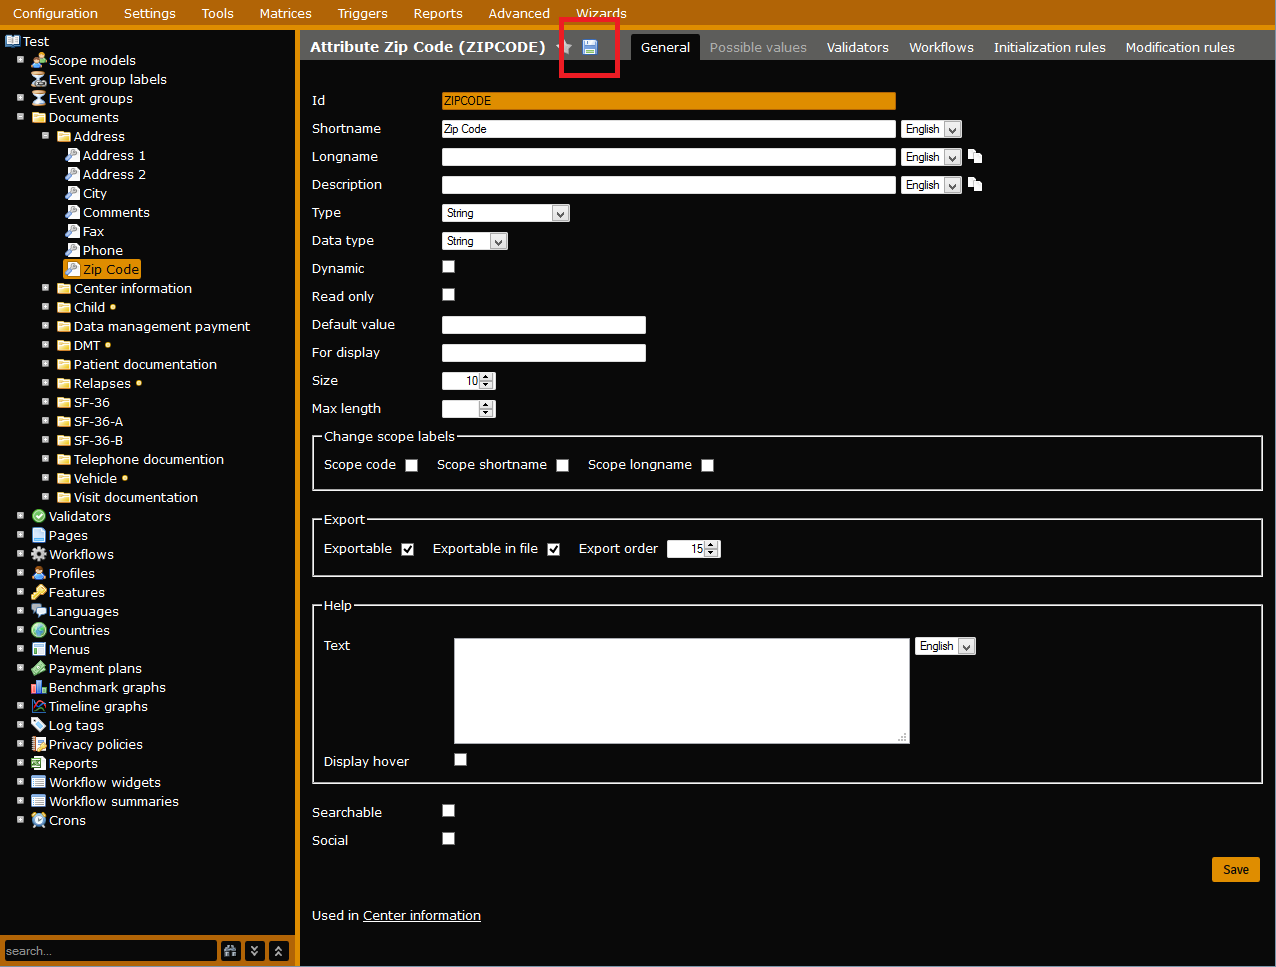
\includegraphics[width=\linewidth]{node_templates_save_template_1}
\end{figure}

After clicking this icon, it is required to set a name and a description for this template. You should also check that the selected repository is "rodano".\\

\begin{figure}[h!]
\caption{Add a name and a description for a template}
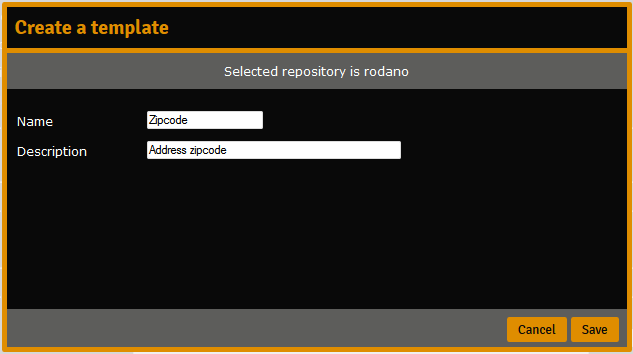
\includegraphics{node_templates_save_template_2}
\end{figure}

\subsubsection{Limitations}
All node information won't be saved in the template. Here are the limitations.

\paragraph{Field model}
All references to validators will be removed. All initialization rules and modifications rules will be removed.

\paragraph{Dataset model}
All field models will be cleaned as described above.

\paragraph{Workflow}
All workflow rules and rules on workflow actions will be removed.

\paragraph{Sheet}
Sheet templates are specific in the way they are a combination of a form model and the dataset model and the field models used in the form model. It is not possible to create a sheet template from a page which is linked to more than one document.

\subsubsection{Restrictions for StudyBuilder}
When creating a template for StudyBuilder, there is also specific restrictions.

\paragraph{Study}
\begin{itemize}
	\item study must contain scope models with id \mbox{"STUDY"}, \mbox{"COUNTRY"}, \mbox{"CENTER"} and \mbox{"PATIENT"}
	\item study must have only one scheduled event group with whose id is "SCHEDULING"
	\item if there is a baseline event model, its id must be "BASELINE" and it must be inside scheduled event group
	\item if there is a screening event model, its id must be "SCREENING" and it must be inside scheduled event group
	\item validators \mbox{"REQUIRED"} and \mbox{"REQUIRED\_WITH\_QUERY"} must exist
	\item profiles \mbox{"INVESTIGATOR"}, \mbox{"DATAMANAGER"}, \mbox{"CRA"}, \mbox{"CRO"} and \mbox{"SPONSOR"} must exist
	\item workflows \mbox{"QUERY"} and \mbox{"PROTOCOL\_DEVIATION"} must exist
	\item workflows \mbox{"EVENT\_SDV"} and \mbox{"PAGE\_SDV"} must exist
	\item workflows \mbox{"PAGE\_ENTRY"}, \mbox{"DATA\_MANAGEMENT"} and \mbox{"EVENTS\_REPORTING"} must exist
\end{itemize}

\subsection{Node template usage}

Node templates which are not studies can be added in any existing configuration.\\

While editing an existing configuration, use the menu Tools\textgreater Templates to go on template management modal window. After selecting the right kind of template in the section on the left, click on the plus icon to add the selected template in the current configuration.\\

\begin{figure}[h]
\caption{Use a template}
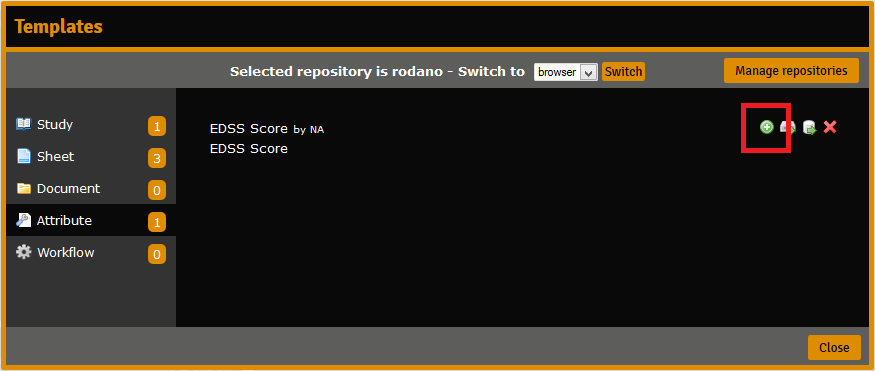
\includegraphics[width=\linewidth]{node_templates_use_template}
\end{figure}

\subsection{Node template deletion}

While editing an existing configuration, use the menu Tools\textgreater Templates to go on template management modal window. After selecting the right kind of template in the section on the left, click on the plus red cross to delete the selected template in the current configuration.\\

\begin{figure}[h]
\caption{Delete a template}
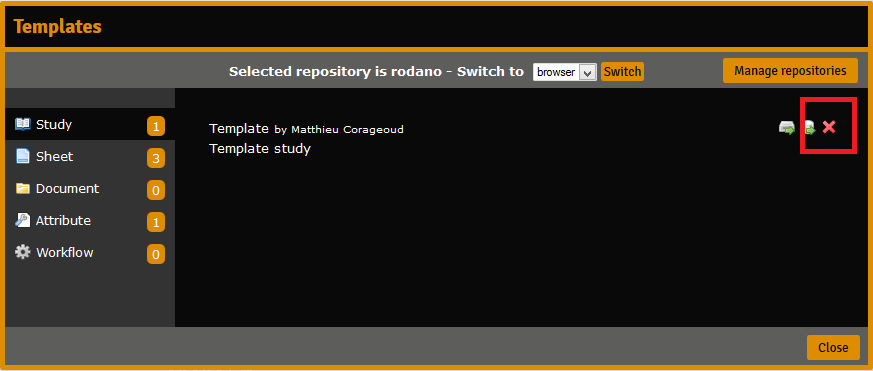
\includegraphics[width=\linewidth]{node_templates_delete_template}
\end{figure}

\subsection{Node template modifications}

The process to edit a node template depends on the kind of templates.

\subsubsection{Templates which are not study}
There is no way to edit these kinds of templates. They must be deleted and re-created.

\subsubsection{Study templates}
Study templates can be edited in KvConfig. In stand-alone mode, use the welcome modal window to load a study from a configured template repository.

\begin{figure}[h]
\caption{Load a study from a repository}
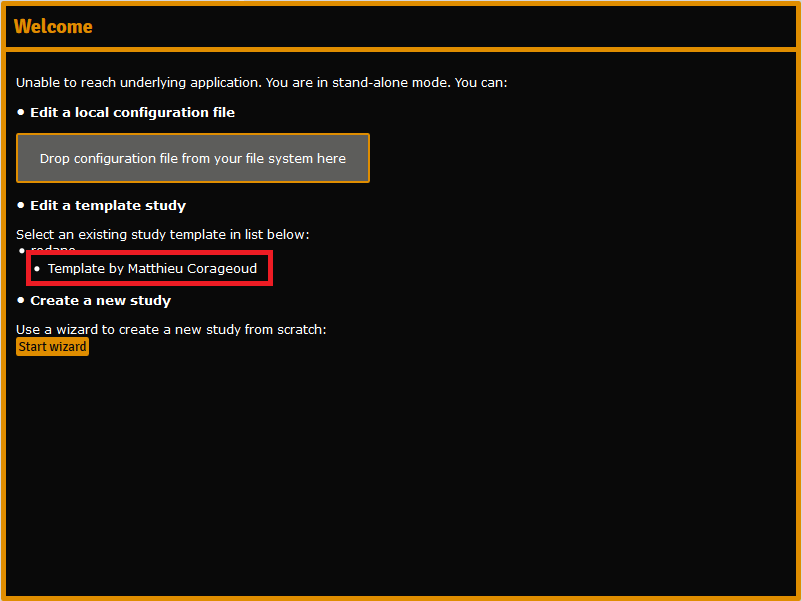
\includegraphics[width=\linewidth]{node_templates_load_study}
\end{figure}

It is then possible to push a template to the template server using menu Configuration\textgreater Push template to server.

\section{Templates usage in StudyBuilder}
StudyBuilder is pre-configured to show study, page and attribute templates from official Rodanotech repository. Every user of the StudyBuilder will have access to templates stored on this server.

\end{document}
